\iffalse
\let\negmedspace\undefined
\let\negthickspace\undefined
\documentclass[journal,12pt,twocolumn]{IEEEtran}
\usepackage{cite}
\usepackage{amsmath,amssymb,amsfonts,amsthm}
\usepackage{algorithmic}
\usepackage{graphicx}
\usepackage{textcomp}
\usepackage{xcolor}
\usepackage{txfonts}
\usepackage{listings}
\usepackage{enumitem}
\usepackage{mathtools}
\usepackage{gensymb}
\usepackage{comment}
\usepackage[breaklinks=true]{hyperref}
\usepackage{tkz-euclide} 
\usepackage{tikz}
\usepackage{circuitikz}
\usepackage{listings}
\usepackage{gvv}                                        
\def\inputGnumericTable{}                                 
\usepackage[latin1]{inputenc}                                
\usepackage{color}                                            
\usepackage{array}                                            
\usepackage{longtable}                                       
\usepackage{calc}                                             
\usepackage{multirow}                                         
\usepackage{hhline}                                           
\usepackage{ifthen}                                           
\usepackage{lscape}
\usepackage{caption}
\newtheorem{theorem}{Theorem}[section]
\newtheorem{problem}{Problem}
\newtheorem{proposition}{Proposition}[section]
\newtheorem{lemma}{Lemma}[section]
\newtheorem{corollary}[theorem]{Corollary}
\newtheorem{example}{Example}[section]
\newtheorem{definition}[problem]{Definition}
\newcommand{\BEQA}{\begin{eqnarray}}
\newcommand{\EEQA}{\end{eqnarray}}
\newcommand{\define}{\stackrel{\triangle}{=}}
\theoremstyle{remark}
\newtheorem{rem}{Remark}
\begin{document}
\parindent 0px
\bibliographystyle{IEEEtran}
\vspace{3cm}

\title{GATE 2022 33.BM}
\author{EE23BTECH11012 - Chavan Dinesh$^{*}$% <-this % stops a space
}
\maketitle
\newpage
\bigskip

\renewcommand{\thefigure}{\arabic{figure}}
\renewcommand{\thetable}{\arabic{table}}
\large\textbf{\textsl{Question:}}
A series $RLC$ circuit with $R = 10 \Omega$, $L = 50 mH$ and $C = 100 \micro F$ connected to
$200$ $V$, $50$ Hz supply consumes power $P$. The value of $L$ is changed such that this
circuit consumes same power $P$ but operates with lagging power factor. The new
value of L is $\hrulefill$ $mH$ (rounded off to two decimal places).
\hfill(GATE 33 BM 2022)

\solution
\fi
\begin{table}[htbp]
    \centering
    \begin{tabular}{|c|c|c|}
\hline
   \textbf{Parameter}  & \textbf{Description} & \textbf{Value}\\
   \hline
   $R$   & Resistance & $10 \Omega$\\
   \hline
  $C$ & Capacitance & $100 \micro F$ \\
  \hline
  $L_{old}$ & Inductor & $50mH$\\
  \hline
  $L_{new}$ & New Inductor &    \\
  \hline
  $Z_{old}$ & Old Impedance & \\
  \hline
  $Z^*$ &New Impedance & \\
  \hline
  
\end{tabular}

    \caption{}
    \label{tab:input_parameters.33.BM.2022}
\end{table}

\begin{figure}[!ht]
    \centering
    \documentclass[tikz, border=2mm]{standalone}
\usetikzlibrary{shapes, arrows.meta}

\begin{document}

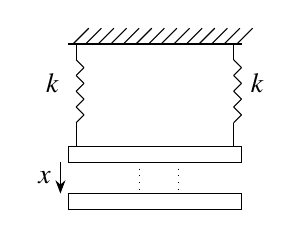
\begin{tikzpicture}
    % Support rod (horizontal)
    \draw (0.4,2) -- (2.6,2); % Shortened the support system
    
    % First Rectangle
    \draw (0.4,0.5) rectangle (2.6,0.7); % Centered the first rectangle
    
    % First Spring (tight rod)
\draw (0.5,1.8) -- (0.5,2);
    \draw (0.5,1.8) -- (0.6,1.7);
    \draw (0.6,1.7) -- (0.5,1.6);
    \draw (0.5,1.6) -- (0.6,1.5);
    \draw (0.6,1.5) -- (0.5,1.4);
    \draw (0.5,1.4) -- (0.6,1.3);
    \draw (.6,1.3) -- (0.5,1.2);
    \draw (0.5,1.2) -- (.6,1.1);
    \draw (.6,1.1) -- (0.5,1);
    \draw (0.5,1)--(0.5,0.7);
    \node at (0.2, 1.5) {$k$};
    
    % Second Rectangle (dotted)
    \draw (0.4,0.1) rectangle (2.6,-0.1);
    
    % Second Spring (tight rod)
    \draw (2.5,1.8) -- (2.5,2);
    \draw (2.5,1.8) -- (2.6,1.7);
    \draw (2.6,1.7) -- (2.5,1.6);
    \draw (2.5,1.6) -- (2.6,1.5);
    \draw (2.6,1.5) -- (2.5,1.4);
    \draw (2.5,1.4) -- (2.6,1.3);
    \draw (2.6,1.3) -- (2.5,1.2);
    \draw (02.5,1.2) -- (2.6,1.1);
    \draw (2.6,1.1) -- (02.5,1);
    \draw (02.5,1)--(02.5,0.7);
    \node at (2.8, 1.5) {$k$};
    
    \foreach \i in {1,...,14}
        \draw ({0.3 + 0.16*\i},2) -- ({0.5 + 0.16*\i},2.2);
    
    \draw[thin, dotted] (1.3,0.5) -- (1.3,0.1);
    \draw[thin, dotted] (1.8,0.5) -- (1.8,0.1);
    
    % Arrow downwards for \delta x
    \draw[->, >=Stealth] (0.3, 0.5) -- node[midway, left] {\(x\)} (0.3, 0.1);
\end{tikzpicture}

\end{document}


    \caption{}
    \label{fig:fig1.33.BM.2022}
\end{figure}

From \figref{fig:fig1.33.BM.2022}

In $s$ - domain,
\begin{figure}[htbp]
    \centering
    \begin{tikzpicture}
\begin{axis}[
    axis lines=middle,
    xmin=-30,
    xmax=30,
    ymin=-0.5,
    ymax=1.5,
    xlabel={$f$},
    ylabel={$H_2(f)$},
    xtick={-15,15},
    ytick={0,1},
    ]
    \addplot [blue, thick] coordinates {(-25,0)(-15,0) (-15,1) (15,1) (15,0)(25,0)};
\end{axis}
\end{tikzpicture}   \label{kk:gateee47Q.2}

\end{figure}

  \begin{align}
      Z = R + sL_{old} + \frac{1}{sC}
  \end{align}
As the circuit consumes same power $P$ but operates with lagging power factor : 

The new impedance($Z^*$) will be :
\begin{align}
    Z^* =  R + sL_{new} + \frac{1}{sC}
\end{align}
Comparing the imaginary parts of the impedances:
\begin{align}
    sL_{old} + \frac{1}{sC} = -\left( sL_{new} + \frac{1}{sC}\right)
    \end{align}
Taking $s = j2\pi f$ :
\begin{align}
     j\left(2\pi fL_{old} - \frac{1}{2\pi fC}\right)  =  -j\left(2\pi fL_{new} - \frac{1}{2\pi fC}\right)
\end{align}
From \tabref{tab:input_parameters.33.BM.2022}:
\begin{align}
    L_{new} \approx 152.7 \text{mH}
\end{align}

% \begin{figure}[ht]
%     \centering
%     \includegraphics[width = \columnwidth]{figs/x_n_stem_plot.png}
%     \caption{}
%     \label{fig:graph1.11.9.3.28}
% \end{figure}


